\newpage
\section{Results}
% General structure.
% Display spectrums, try to calculate quality factor at least.
% Display some prelimary purities.
% Some stuff I probably should have calculated:
% Powers in the waveguide, peak power
\subsection{Glassgow}
This chip was used to do an initial proof of concept that the JSI of a ring resonator could be measured at high resolution. Here the aim was to explore different ring geometries and develop an intuition on how to do the experiment. The Pritel pulsed laser was used with a pulse duration of \SI{2}{\pico\second}, a FWHM of \SI{1.0}{\nano\meter} with wavelength range \SI{1530}{\nano\meter} to \SI{1530}{\nano\meter} and a peak power of \SI{100}{\watt}. Due to the pulsed laser sometimes destroying the spot size converter on the chip a \SI{3}{\decibel} attenuator was added just after the laser output, this resulted in roughly about \SI{5}{\deci\bel\m} of power coming out of the lens fiber.

\begingroup
    \centering  
    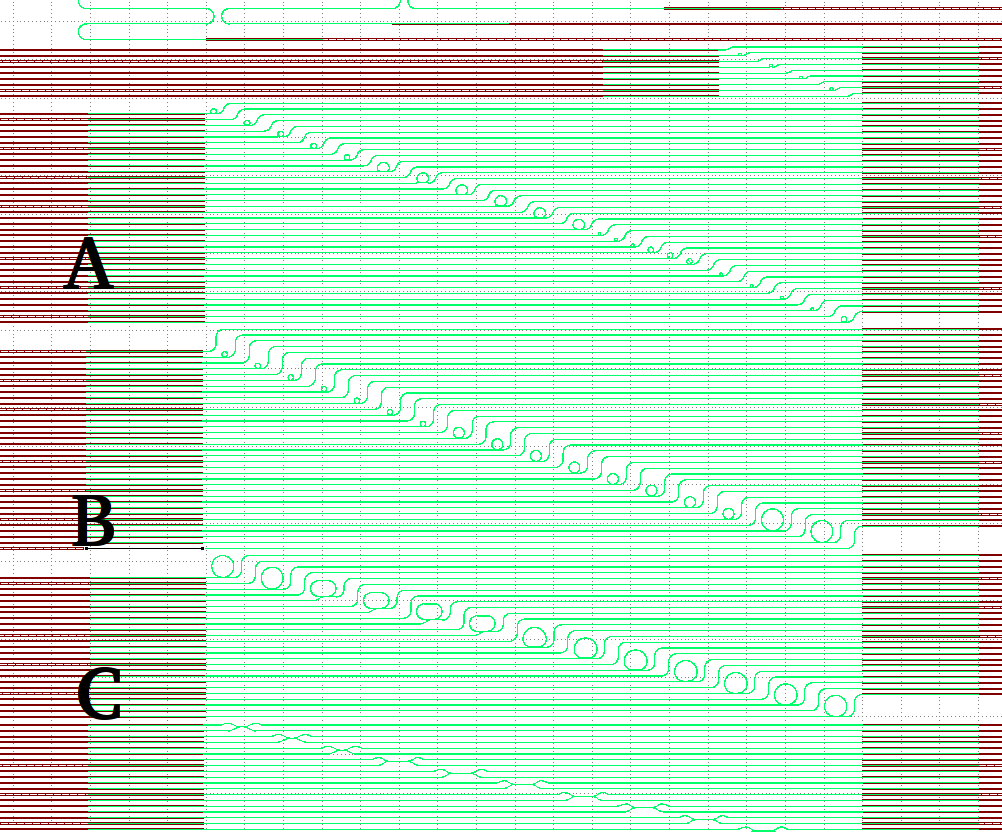
\includegraphics[width=10cm]{img/method/glassgowChipNumbering.png}
    \captionof{figure}{Glassgow test structure chip}
     \vspace{3pt} \label{glassgowChip}
\endgroup

As each device on the chip has unique characteristics due to fabrication errors only some devices produced good data meaning that a full characterisation of the chip was not possible and only a few devices were used. Typically it was imperfections in the spot size converters on the chips being which prevented good JSI's from being collected but another issue encountered was under coupling of the rings.

Here we present three data sets collected, each has high SNR of at least $20$ allowing for the maximum purity $P_{max}$ to be calculated with high accuracy. The relevant spectral scan is presented with the JSIs for reference, these are routine scans performed with the tunable CW laser typically at \SI{1}{\m\watt} of which roughly \SI{-14}{\deci\bel\m} gets into the chip. 

% RING C17
\begingroup
    \centering  
    \includegraphics[width=15cm]{/home/luka/Dropbox/cqp/report/thesis/res/glassgow/C17/graph.pdf}
    \captionof{figure}{{\bf JSI Ring C17} We calculate a quality factor of $Q \approx 25000$. In this instance the coupling loss was on average \SI{20}{\dB} and the input power of the pulsed laser was \SI{5.1}{\dB} giving a estimated power in waveguide of \SI{-5}{\dB}. The probe laser operated at \SI{1}{\m\watt}. Fitting the spectral scans of the ring resonators gives coupling parameters of the order $r=0.946$ $\tau = 0.985$ $n_{eff} = 4.136$, note these are only estimates.} 
     \vspace{3pt} \label{c17_jsi}
\endgroup

% C17 key points
% it works, SW stuff interferes and is of lower intensity, it happens before the ring


Figure \ref{c17_jsi} shows a clear response from the ring resonator at the resonant frequencies, superimposed on this there is also straight waveguide stimulated four wave mixing observed at much lower intensities. It can be deduced that much of this straight wave guide contribution happens before the ring as it is filtered at the resonance wavelength.
The asymmetry is an experimental artefact of imperfect alignment of the resonances with the AWG channels and the pump laser. This is  $P_{max}$ value.

% RING C21
\begingroup
    \centering  
    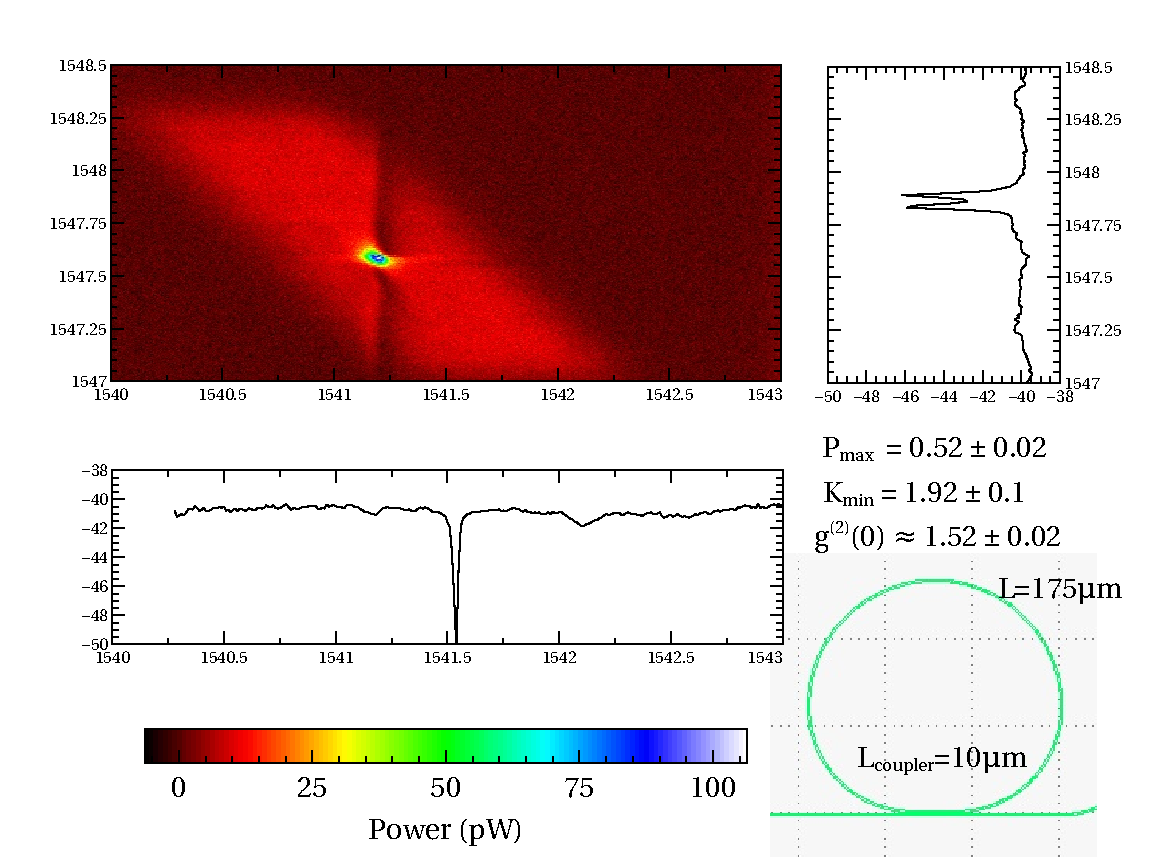
\includegraphics[width=15cm]{/home/luka/Dropbox/cqp/report/thesis/res/glassgow/C21/c21graph.pdf}
    \captionof{figure}{{\bf JSI Ring C21} We calculate a quality factor of $Q \approx 28000$. In this instance the coupling loss was on average \SI{21}{\dB} and the input power of the pulsed laser was \SI{5.5}{\deci\bel\m} giving a estimated power in waveguide of \SI{-5}{\deci\bel\m}. The probe laser operated at \SI{1}{\m\watt}. Fitting the spectral scans of the ring resonators gives coupling parameters of the order $r=0.957$ $\tau = 0.977$ $n_{eff} = 4.144$, note these are only estimates.} 
     \vspace{3pt} \label{c21_jsi}
\endgroup

In figure \ref{c21_jsi} we see ring C21 which has has many physical similarities with ring C17 shown in figure \ref{c17_jsi} however we observe a few key differences. Firstly the resonance that the CW laser probes is split but this is not reflected in the JSI because the split feature is on the order of \SI{0.01}{\nano\meter} which under the \SI{0.03}{\nano\meter} resolution of the OSA. This inability to resolve finer features which are almost certainly encoded in the real JSA is an important topic discussed later on in this work.

Secondly the coupling distance of the egg shaped resonator is slightly shorter here which is reflected in a slightly smaller value for $r$, however this difference isn't significant enough to use for a comparison as there are many other factors between the two experiments that were not held constant, in particular the alignment of the AWG channels.

% RING B32
\begingroup
    \centering  
    \includegraphics[width=15cm]{/home/luka/Dropbox/cqp/report/thesis/res/glassgow/B32/graph.pdf}
    \captionof{figure}{{\bf JSI Ring B32} We calculate a quality factor of $Q \approx 14000$. In this instance the coupling loss was on average \SI{22}{\deci\bel\m} and the input power of the pulsed laser was \SI{5.1}{\deci\bel\m} giving a estimated power in waveguide of \SI{0}{\deci\bel\m}. The probe laser operated at \SI{1}{\m\watt}. Fitting the spectral scans of the ring resonators gives coupling parameters of the order $r=0.985$ $\tau = 0.947$ $n_{eff} = 4.136$, note these are only estimates. } 
     \vspace{3pt} \label{b32_jsi}
\endgroup

The final JSI collected for this chip is shown in figure \ref{b32_jsi}, here the ring geometry is of the more traditional circular shape. It is observed that the resonance has some asymmetry due to more prominent non-linear effects. We observe the intensities of the ring resonator and straight wave guide FWM processes to be more similar in this scan which can be accounted for by the lower quality factory. Again it is notable to see that the ring seems to be collecting some of the straight wave guide FWM, however at a shifted frequency to the peak of the ring FWM, this is contradictory to the two previous examples and may be due to the more non-linear response of this ring.
\newline\newline
\noindent
{\bf Summary }The three purities observed $(0.42,0.52,0.62)$ coincide with previous characterisations of the chip using the single photon detectors which measured a purity of on the order 0.45 \cite{scammell_indistinguishable_2014}. A advantage to these measurements is they allow one to easier develop ways of increasing the purity.
\subsection{a-Si}


Here the power scan method developed in section \ref{powerScan} was applied to an amorphous silicon chip. This chip contained ring resonator and straight waveguide test structures which were coupled via diffraction gratings, requiring vertical coupling. This chip was chosen because of pre-existing analysis of the pair generation rate and of the purity using the methods from section \ref{g2method}. Figure \ref{aSIChip} shows an example of a ring resonator structure on the chip.

\begingroup
    \centering  
    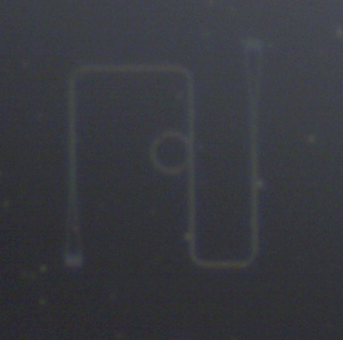
\includegraphics[width=5cm]{img/method/chipPictures/exampleASIRing.png}
    \captionof{figure}{Example of a ring resonator structure on the a-Si chip.}
     \vspace{3pt} \label{aSIChip}
\endgroup

The Pritel pulsed laser had a pulse duration of \SI{5}{\pico\second}, a FWHM of \SI{0.4}{\nano\meter} with wavelength range \SI{1530}{\nano\meter} to \SI{1560}{\nano\meter}, a peak power of \SI{50}{\watt} and a repetition rate of \SI{50}{\mega\hertz}. In this experiment it was decided that due to the temperature and coupling variations in the set up, the $g^{(2)}(0)$ measurement and the JSI would be collected at as close to the same time as possible. This meant that the set up was alternated in between the two methods for each different value of the variable attenuator, this resulted in a rather complex experimental procedure.

The ring chosen had $Q \approx 7000$, $r$ and $\tau$ values of (0.98,0.93), noting that due to their symmetry it was not possible to discern which one is which without further analysis, so it was possible the ring was under coupled. The ring has a diamter of \SI{26.5}{\micro\m} and is coupled to a \SI{550}{\micro\m} long bus waveguide

The Pritel erbium-doped fiber amplifier (EDFA) was used to increase the output power of the laser. Doing this well was not a trivial task as at high powers self modulation (SPM) occurs in the fiber optic cables, particularly as the DWDMs contained large lengths of fiber. So a amplification level was found which minimised SPM while still offering a worthwhile amplification. Also in order to reduce the ASE which would drown out the joint spectrum signal, a further DWDM was placed at the output of the laser to avoid amplifying its ASE output in the EDFA.

The results of the joint spectrum scans are shown in figure \ref{asi_jsi_grid}, three filters have been applied to the data in order to remove noise. These are:


% asi
\begingroup
    \centering
    \includegraphics[width=16cm]{/home/luka/Dropbox/cqp/report/thesis/res/asi/graph.pdf}
    \captionof{figure}{From high power to low power (see figure \ref{theshit} for the purity and power values.) the joint spectrums collected in the experiment. The VBW was set to 10Hz, with a point average of 30, resolution of 0.03nm on the OSA and a resolution of 0.01nm on the CW. The coupling was adjusted so that the lose as as close to \SI{19}{\decibel} as possible.}
     \vspace{3pt} \label{asi_jsi_grid}
\endgroup

The results show a visible change in shape at different powers, looking at \ref{theShit} the purities do somewhat match up with 

\begingroup
    \centering
    \includegraphics[width=10cm]{res/asi/averageAndJS.pdf}
    \captionof{figure}{A comparison of the two experiments, the $g^{(2)}(0)$ values come from an average of the data in figure \ref{lizzylizzy}. We know that the JSI only gives an upper bound for the  purity, this is confirmed here. The error bars for the JSI method are derived using figure \ref{noiseGraph}, where noise was added to a simulation and the error in the purity is numerically found as a function of SNR. Here the SNR's were between 1.5 and 2.5 hence the large error bars.}
     \vspace{3pt} \label{theshit}
\endgroup

\begingroup
    \centering
    \includegraphics[width=10cm]{/home/luka/Dropbox/cqp/report/thesis/res/asi/g2AndTrio.pdf}
    \captionof{figure}{This data was collected by Lizzy Hemesley. Experiment 2 was done in conjunction with the JSI experiment.} 
     \vspace{3pt} \label{lizzylizzy}
\endgroup
